\newpage

\section{Właściwości}

\subsection{Siarczek galu}
Struktura pasmowa i przerwa energetyczna to są kluczowe parametry dla półprzewodników chalkogenowych. \textit{Chalkogenki} – nieorganiczne związki chemiczne, w których anionami są chalkogeny, tj. siarczki, selenki i telurki. Przykładowymi chalkogenkami są związki $\mathbf{GaS}$, $\mathbf{Ga_{2}S_{3}}$, $\mathbf{GaSe}$, $\mathbf{Ga_{2}Se_{3}}$, które należą do związków III-VI (III: \textbf{In}, \textbf{Ga} i VI: \textbf{S}, \textbf{Se}, \textbf{Te}) grupy chemicznej. Związek $\mathbf{Ga_{2}S_{3}}$ jest ważnym członkiem związków III-VI , który może posiadać najszerszą lukę w zespole. Nieścisłość pomiędzy atomami III i VI grup powoduje, że związek ma różne stechiometrie, zróżnicowane fazy krystaliczne i różne formy sieci.

$\mathbf{GaSe}$ i $\mathbf{GaS}$ mogą krystalizować się w sześciakątnej strukturze warstwowej, ale w tych związkach warstwy różnie układają się w stos. $\mathbf{GaSe}$ posiada prostą przerwę energetyczną wynoszącą około 2 eV. Podczas gdy materiał $\mathbf{GaS}$ staje się przewodnikiem ze skośną przerwą energetyczną o wartości 2.53 eV.

$\mathbf{Ga_{2}Se_{3}}$ może posiadać wadliwą strukturę blendy cynkowej, w której 1/3 miejsc kationowych jest pusta (położenie pustych miejsca jest losowe w siatce krystalicznej) jest to oczywiście zdefektowany półprzewodnik z prostą przerwą energetyczną o wartości 2-2.4eV.

Chalkogenki $\mathbf{GaSe}$, $\mathbf{GaS}$, $\mathbf{Ga_{2}Se_{3}}$ mają wartości przerwy energetycznej poniżej 2.55 eV. które mogą być zakatologowane do materiałów w zakresie widzialnyma, ale nie do zastosowań w zakresie UV jak związek $\mathbf{Ga_{2}S_{3}}$

Siarczek galu występuje w dwóch postaciach:
\begin{itemize}
	\item Siarczek galu(II) - $\mathbf{GaS}$
	\item Siarczek galu(III) - $\mathbf{Ga_{2}S_{3}}$
\end{itemize}
%grupa przestrzenna $\mathbf{P\;6_{3}/mmc}$
$\mathbf{GaS}$ tworzy bezbarwne lub żółte kryształki układu heksagonalnego. Kryształ siarczku galu $\mathbf{(GaS)}$ należy do rodziny półprzewodników warstwowych III-VI. Krystalizuje się w sześciokątnej strukturze o parametrach sieci $a = 0,3578$ i $c = 1,547$ nm. Każda warstwa w strukturze krystalicznej składa się z dwóch atomów galu i dwóch atomów siarki ułożonych w stos wzdłuż osi $c$ z powtarzającą się jednostką $\mathbf{S-Ga-Ga-S}$.
\begin{figure}[H]
	\begin{center}
		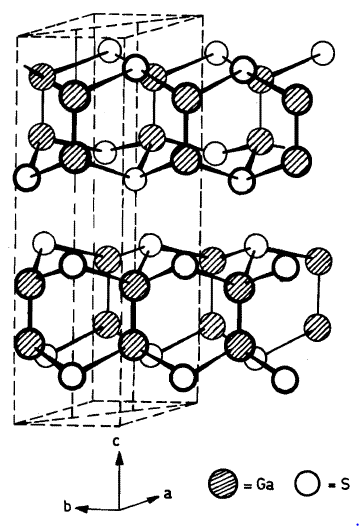
\includegraphics[width=0.35\linewidth]{Wlasciwosci/GaS_Schematic_Structure.png}
		\caption{Schematyczna reprezentacja struktury krystalicznej $\mathbf{GaS}$ [1]}
	\end{center}
\end{figure}

W kryształach $\mathbf{GaS}$ dominują słabe siły van der Waalsa w oddziaływaniach międzywarstwowych. Silne kowalencyjne siły dominują w oddziaływaniach wewnątrzwarstwowych.
$\mathbf{GaS}$ to półprzewodnik szerokopasmowy, który jest obiecującym materiałem. Skośna przerwa energetyczna wynosi $2.5eV$, a prosta wynosi $2.95eV$. Materiał umożliwia
wytwarzanie niebieskich urządzeń emitujących światło [1].

$\mathbf{Ga_{2}S_{3}}$ jest również półprzewodnikiem zdefektowanym z powodu niedopasowania Ga – III i S - VI. Jedna trzecia miejsc kationowych, czyli pozycji galowych nie jest zajęte. Występują luki kationowe, które znacznie wpływają na właściwości fizyczne tego materiału i jego obszar zastosowań. Może mieć następne struktury krystaliczne: jednoskośna, sześciokątna, kubiczna. Najbardziej stabilną i ogólnie znajdowaną strukturę krystaliczną jest struktura jednoskośna.

\textit{Faza $\alpha'$-$Ga_{2}S_{3}$ i $\alpha$-$Ga_{2}S_{3}$} \\
Najbardziej stabilną fazą związku $\mathbf{Ga_{2}S_{3}}$ jest faza $\alpha'$-$Ga_{2}S_{3}$. Ma jednoskośny układ krystalograficzny. Związek $\alpha'$-$Ga_{2}S_{3}$ ma prostą przerwę energetyczną o wartości 3.05 - 3.30 (w zależności od źródła) eV i skośną przerwę energetyczną o wartości 3.4 eV. Wyhodowane kryształki są jasnożółte lub przezroczyste. Powodem występowania żółtego koloru w tym półprzewodniku, gdzie przerwa energetyczna ma energię większą niż najbardziej energetyczny foton światła widzialnego, jest obecność luk kationowych. Luki w pasmie energetycznym zlokalizowane na poziomie 0.8 - 0.9 eV wyżej od najwyższego punktu pasma walencyjnego. Te luki tworzą pułapki elektronowe. Elektrony które przechodzą z pasma przewodnictwa do tych pułapek emitują fotony o energii 2.15 - 2.25 eV co odpowiada światłu żółtemu.

Faza $\alpha'$-$Ga_{2}S_{3}$ może posiadać dwie grupy przestrzenne. Parametry komórki elementarnej dla tego materiału w zależności od grupy przestrzennej wynoszą:
\begin{itemize}
	\item Grupa przestrzenna $Cc$ - $a=1.111\;nm$, $b=0.640\;nm$, $c=0.702\;nm$, $\beta=121.17^{\circ}$;
	\item Grupa przestrzenna $Bb$ -  $a=1.109\;nm$, $b=0.958\;nm$, $c=0.640\;nm$, $\beta=141.15^{\circ}$;
\end{itemize}

Grupa przestrzenna dla fazy $\alpha$-$Ga_{2}S_{3}$ jest $P6_1$. Ta faza ma sześciokątny układ krystalograficzny. Parametry komórki elementarnej $a=0.639\;nm$, $c=1.804\;nm$.

\begin{figure}[H]
	\begin{center}
		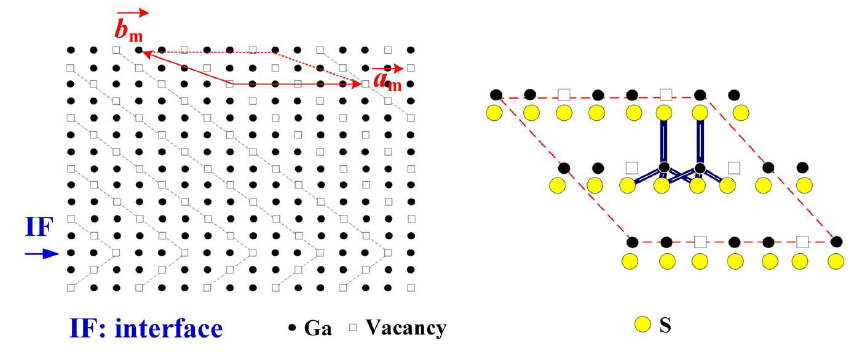
\includegraphics[width=1.0\linewidth]{Wlasciwosci/Przekroj_Ga2S3.png}
		\caption{Na lewym rysunku przedstawiono zdefektowaną sieć krystaliczną w płaszczyźnie prostopadłej do osi c dla związku $\alpha'$-$Ga_{2}S_{3}$. Kationowe luki tworzą interfejs. Na prawym rysunku pokazano sposób ułożenia i wiązania atomów. Cztery aniony S w wierzchołkach czworościanu i w środku jeden kation $\mathbf{Ga}$ lub luka.}
	\end{center}
\end{figure}

\textit{Faza $\beta$-$Ga_{2}S_{3}$} \\
Ta faza jest nazywana fazą $\beta$, z sześciokątnym układem krystalograficznym. Grupa przestrzenna $P6_{3}mc$ Parametry komórki elementarnej: $a=0.368\;nm$,  $c=0.602\;nm$. Faza $\beta$ związku $Ga_{2}S_{3}$ ma najmniejszą przerwę energetyczną dla tego materiału 2.48 eV.

\textit{Faza $\gamma$-$Ga_{2}S_{3}$} \\
Faza z grupą przestrzenna $F-43m$. To jest niskotemperaturowa faza. Kryształki $\gamma$-$Ga_{2}S_{3}$ są białego koloru. Przerwa energetyczna wynosi 2.96 eV. Parametry komórki elementarnej: $a=0.517\;nm$.

\begin{table}[H]
	\begin{tabular}{|c|c|c|c|c|}
		\hline
		\multicolumn{1}{|l|}{\textbf{Nazwa}} & \textbf{\begin{tabular}[c]{@{}c@{}}Układ \\ krystalograficzny\end{tabular}} & \textbf{\begin{tabular}[c]{@{}c@{}}Grupa\\ przestrzenna\end{tabular}} & \textbf{Typ struktury}                                            & \textbf{\begin{tabular}[c]{@{}c@{}}Parametry sieci\\ krystalicznej\end{tabular}} \\ \hline
		$\alpha$-$\mathbf{Ga_{2}S_{3}}$                              & Sześciokątny                                                                & $P6_{1}$                       & \begin{tabular}[c]{@{}c@{}}Superstruktura \\ wurcytu\end{tabular} & $a=0.639\;nm$,$c=1.804\;nm$                                                                   \\ \hline
		\multirow{2}{*}{$\alpha'$-$\mathbf{Ga_{2}S_{3}}$}            & \multirow{2}{*}{Jednoskośny}                                                & $Cc$                          & \begin{tabular}[c]{@{}c@{}}Superstruktura\\ $\alpha$-$\mathbf{Ga_{2}S_{3}}$\end{tabular}  & 
		\begin{tabular}[c]{@{}c@{}}$a=1.111\;nm$, $b=0.640\;nm$,\\ $c=0.702\;nm$,$\beta=121.17^{\circ}$\end{tabular}                                                                            \\ \cline{3-5} 
		&                                                                             & $Bb$                          & \begin{tabular}[c]{@{}c@{}}Superstruktura\\ $\alpha$-$\mathbf{Ga_{2}S_{3}}$\end{tabular}  & 	
		\begin{tabular}[c]{@{}c@{}}$a=1.109\;nm$, $b=0.958\;nm$,\\ $c=0.640\;nm$, $\beta=141.15^{\circ}$\end{tabular}                                                                            \\ \hline
		$\beta$-$\mathbf{Ga_{2}S_{3}}$                              & Sześciokątny                                                                & $P6_{3}mc$                     & Wurcyt                                                            & $a=0.368\;nm$,                                                                                           $c=0.602\;nm$                                                                              \\ \hline
		$\gamma$-$\mathbf{Ga_{2}S_{3}}$                              & Sześcienny                                                                  & $F$-$43m$                       & Blenda cynkowa                                                    & $a=0.517\;nm$                                                                            \\ \hline
	\end{tabular}
	\caption{Wszystkie fazy krystaliczne $\mathbf{Ga_{2}S_{3}}$}
\end{table}

Główne piki na widmie rentgenowskim dla każdej z faz występują pod tymi samymi kątami, jedynie intensywności mają różne. To oznacza że jeżeli Faza kubiczna $\gamma$-$Ga_{2}S_{3}$ ma strukturę blendy cynkowej $\mathbf{ZnS}$ ze zdefektowaną podsiecią kationową, to i każda z faz też będzie miała zdefektowaną podsieć kationową.

\begin{figure}[H]
	\begin{center}
		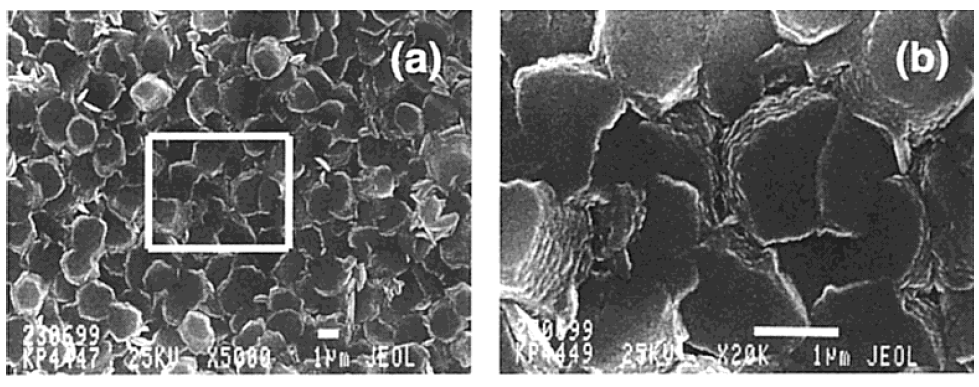
\includegraphics[width=1.0\linewidth]{Wlasciwosci/SEM_Ga2S3.png}
		\caption{Na tym rysunku są przedstawione zdjęcia $\alpha$-$Ga_{2}S_{3}$ za pomocą SEM przy powiększeniu : a) 5000 razy, b) 20000 razy.}
	\end{center}
\end{figure}

\subsection{Zastosowania $\mathbf{Ga_{2}S_{3}}$}

Jednym z najważniejszych problemów materiałów półprzewodnikowych stosowanych w fotoelektronice jest opracowanie związków o stabilnych właściwościach pod wpływem promieniowania UV, promieniowania rentgenowskiego i $\gamma$, a także opracowanie detektorów promieniowania jonizującego w oparciu o te materiały. Strukturalne defekty w materiale wywoływane są pod wpływem promieni UV, promieniowania rentgenowskiego i $\gamma$. Koncentracja i rodzaj tych defektów zależy zarówno od dawki promieniowania, jak i rodzaju materiału. Detektory promieniowania rentgenowskiego i promieniowania UV oparte na tych materiałach muszą spełniać warunek, że koncentracja ich własnych defektów jest znacznie wyższa niż koncentracja defektów wywołanych promieniowaniem. Materiały takie jak $\mathbf{A_{2}^{III}C_{3}^{VI}}$, szczególnie $\mathbf{Ga_{2}S_{3}}$, spełniają to wymaganie. $\frac{1}{3}$ pozycji w podsieci kationowej są nieobsadzone i tworzą luki, czyli defekty kryształu. Koncentracja własnych defektów w tych materiałach wynosi około $10^{22}\;cm^{-3}$. Przewodność elektryczna pojedynczych kryształów $\mathbf{Ga_{2}S_{3}}$ w normalnej temperaturze wynosi około $10^{-12}\;\Omega^{-1}cm^{-1}$. Przewodność elektryczna wzrasta 3 razy z domieszką $\mathbf{Cd}$.

Domieszkowany (Cr i Fe) i niedomieszkowany Ga2S3 może być materiałem luminescencyjnym z emisją fal o długości od bliskiej podczerwieni do UV.

$\mathbf{GaS}$ długi czas zajmował wysoką pozycję wśród materiałów do aplikacji THz. Ma bardzo szerokie okna dla 0.62 – 20 $\mu m$ i od 50 $\mu m$ – do THz. Ale jego warstwowa struktura i wynikające z tego słabe właściwości mechaniczne ograniczają możliwości zastosowania tego materiału. $\mathbf{Ga_{2}S_{3}}$ jest przezroczysty dla 0.44 – 25 $\mu m$ co jest pokazano na wykresie poniżej:

\begin{figure}[H]
	\begin{center}
		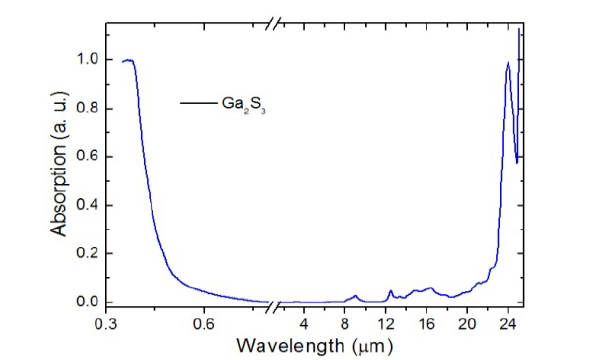
\includegraphics[width=0.8\linewidth]{Wlasciwosci/Widmo-absorpcji-Ga2S3.png}
		\caption{Widmo absorpcji dla $Ga_{2}S_{3}$.}
	\end{center}
\end{figure}

Materiał $\mathbf{Ga_{2}S_{3}}$ ma zastosowanie optyczne i optoelektroniczne (diody elektroluminescencyjne (LED), absorber UV w fotowoltaicznych urządzeniach, generator drugiej harmonicznej, generator trzeciej harmonicznej np. w materiale $\mathbf{Ti_{2}S}$-$\mathbf{Ga_{2}S_{3}}$-$\mathbf{GeS_{2}}$), ze względu na swoją skośną i szeroką przerwę energetyczną). (duże czyli bulk kryształy) Struktura cienkowarstwowa Ga2S3/In/Ga2S3 ma potencjalne zastosowanie jako rezonator mikrofalowy. Jego dwójłomność 0,025 jest większa niż $\mathbf{CdSe}$, która pozwala dopasować fazę SHG dla długości fali dłuższej niż 1910 $\mu m$.

Kolejne z możliwych zastosowań tego materiału jest pasywacja powierzchni półprzewodnikowej III - V tj. do utworzenia "natywnej" warstwy siarczkowej na $\mathbf{GaAs}$ lub $\mathbf{InP}$ poprzez siarkowanie na powierzchni; tak, że rekombinacja powierzchni $\mathbf{GaAs}$ lub $\mathbf{InP}$ można radykalnie stłumić, co z kolei znacząco poprawia wydajność urządzenia W dziedzinie nauki o materiałach i technologii brakuje skutecznych warstw pasywacji powierzchniowej  dla $\mathbf{GaAs}$.

Materiały $\mathbf{GaS}$ i $\mathbf{Ga_{2}S_{3}}$ mają doskonałe właściwości dla soczewek optycznych, optycznych amplifikacji do telekomunikacji i produkcji laserowej i są nietoksyczne.

\subsection{Widmo ramanowskie i polaryzacyjne}

Widmo ramanowskie dla związku $\alpha$-$\mathbf{Ga_{2}S_{3}}$ ma 7 pików, które odpowiadają przesunięciom: 1) 119, 2) 135, 3) 148, 4) 238, 5) 309, 6) 331, 7) 392 $cm^{-1}$. Znaczące piki takie jak 1), 2) i 3) (Ga-S2 are mainly due to the Ga-S2 scissoring) 
the band at 238 cm-1 is due to the ring out plane bending of (alfa-Ga2S3). The presence of Ga-S symmetric starching is clearly identified with the large intense spectral band at 392.4 cm-1. \textbf{nie wiem co to znaczy}.

\begin{figure}[H]
	\begin{center}
		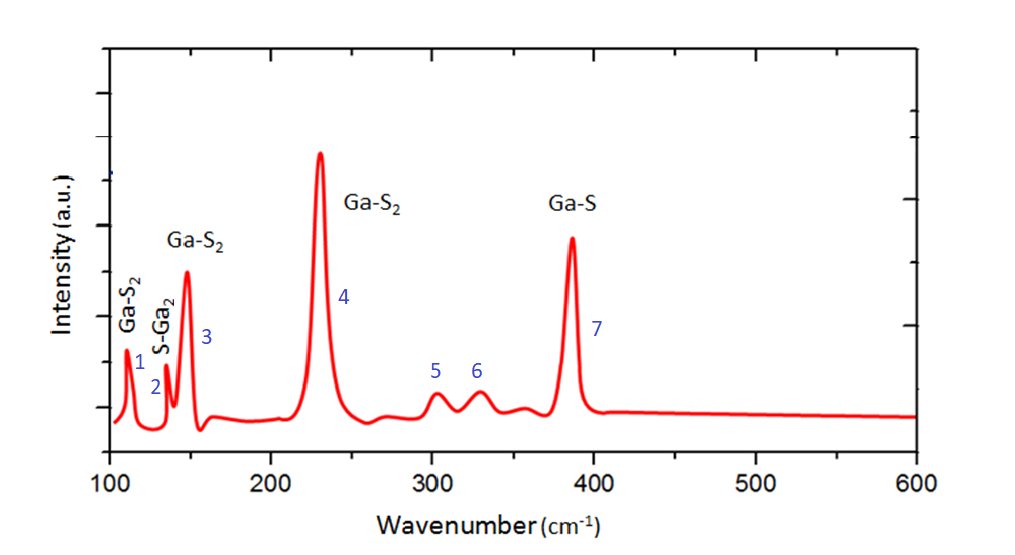
\includegraphics[width=1.0\linewidth]{Wlasciwosci/Raman-Ga2S3.png}
		\caption{Widmo ramanowskie dla $\alpha$-$Ga_{2}S_{3}$}
	\end{center}
\end{figure}

W zależności od kierunku polaryzacji światła laserowego, które oddziałuje z fononami w materiale intensywności pików będą się zmieniać. Po zaobserwowaniu tych zmian można uzyskać widmo polaryzacyjne. Przykładowe widmo polaryzacyjne znajduje się poniżej:
 
\begin{figure}[H]
	\begin{center}
		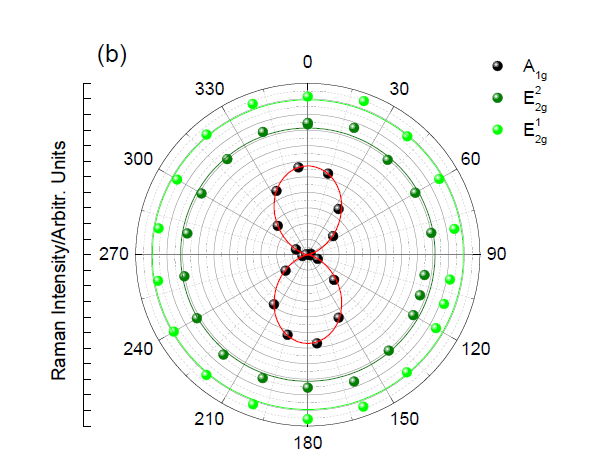
\includegraphics[width=0.8\linewidth]{Wlasciwosci/Spectre-polarization-Ga2S3.png}
		\caption{Przykładowe widmo polaryzacyjne dla trzech pików $\mathbf{A_{1g}}$ $\mathbf{E_{2g}^{2}}$ $\mathbf{E_{2g}^{1}}$. Tu intensywność czyli pole powierzchni piku to odległość od środka do punktu, który odpowiada określonemu kątowi. Ten kąt jest kątem między kierunkiem drgania dipola a promieniowaniem pobudzającym. Widać, że tylko pik $\mathbf{A_{1g}}$ znacząco reaguje na zmianę polaryzacji.}
	\end{center}
\end{figure}

Intensywność piku Ramanowskiego można pokazać taką relacją:
\begin{equation}
	I_{s} \sim |e_{i}\mathbf{R}e_{s}|^{2}
\end{equation}
\begin{itemize}
	\item $e_{i}$ i $e_{s}$ - wwektory polaryzacji promieniowania podającego i rozproszonego odpowiednio.
	\item $\mathbf{R}$ - Tensor ramanowski, który zależy od symetrii kryształu i konkretnego drgającego modu.
\end{itemize}

Wyznaczenie tensorów ramanowskich dla związku $\alpha$-$Ga_{2}S_{3}$ i jest celem tej pracy.



